\chapter{Supplemental Material for Chapter \ref{chap:chapter2}}

%%%%%%%%%%%%%%%%%%%%%%%%%%%%%%%%%%%%%%%%%%%%%%%%%%%%%%%%%%%%%%%%%%%%%%%%%%%%%%%%
\section{Supplementary Figures}
%%%%%%%%%%%%%%%%%%%%%%%%%%%%%%%%%%%%%%%%%%%%%%%%%%%%%%%%%%%%%%%%%%%%%%%%%%%%%%%%

\begin{figure}[h]
    \centering
    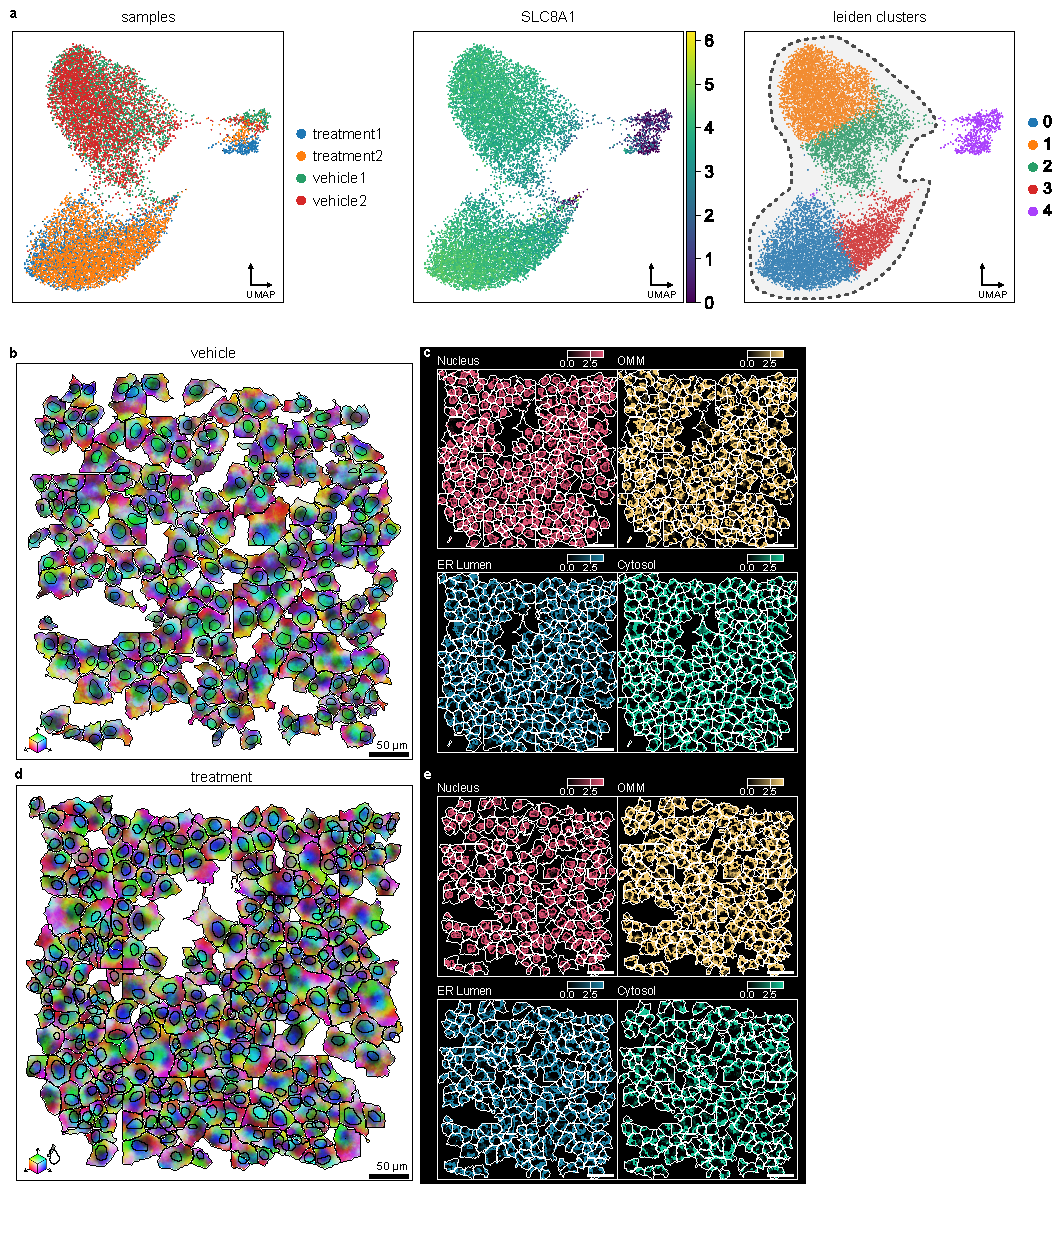
\includegraphics[width=\textwidth]{2_figures-and-files/FigS1.pdf}
    \caption[Filtering and RNAflux analysis of DOX treated cardiomyocytes.]{\textbf{Filtering and RNAflux analysis of DOX treated cardiomyocytes.} A. Left: UMAP of all 4 cardiomyocyte samples, colors denote different samples. Center: Cells are colored by log-scaled SLC8A1 RNA expression. Right: Leiden clustering identifies 5 clusters, separating low expression SLC8A1 into cluster 4. Representative crop of B. vehicle and D. treatment samples, colored by the first 3 principal components of its RNAflux embedding. Relative enrichment of transcripts enriched for location-specific expression in C. vehicle and E. treatment samples. Red, yellow, blue and green enrichment correspond to nuclear, OMM, ER lumen, and cytosol genesets respectively. }\label{fig:supplement cardio filtering and rnaflux}
\end{figure}
